\chapter{Configuración y mantenimiento de \ReplicaGenOne{}}\label{ch:replica-setup}

Este capítulo se aplica al cuadro clásico \ReplicaGenOne{} mostrado en \autoref{fig:replica-classic}. Si su tablero coincide con la disposición de \ReplicaNextLong{}, consulte el capítulo anterior.

\begin{figure}[htbp]
    \centering
    \begin{subfigure}{0.46\textwidth}
        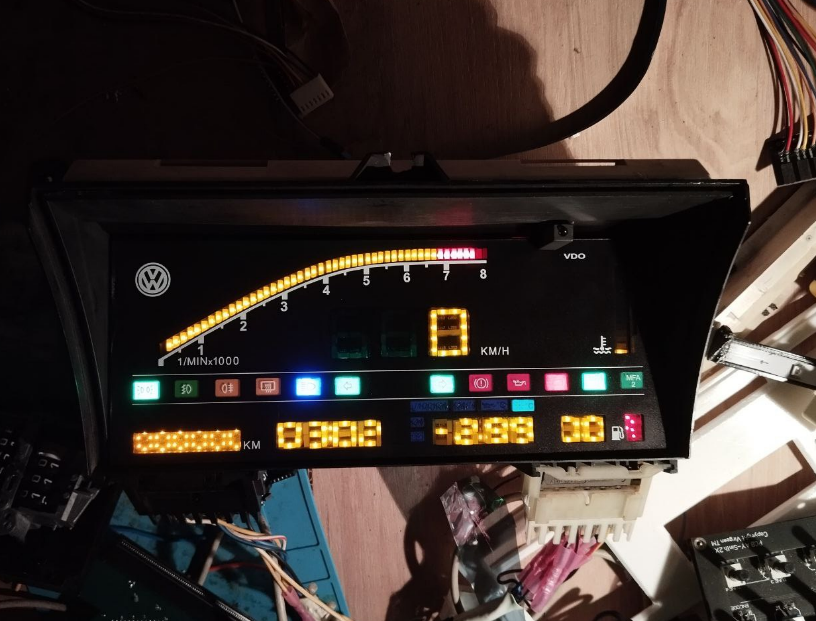
\includegraphics[width=\linewidth]{digifiz_manual/image046.png}
        \caption{Classic \ReplicaGenOne{} with square bezel.}
    \end{subfigure}\hfill
    \begin{subfigure}{0.46\textwidth}
        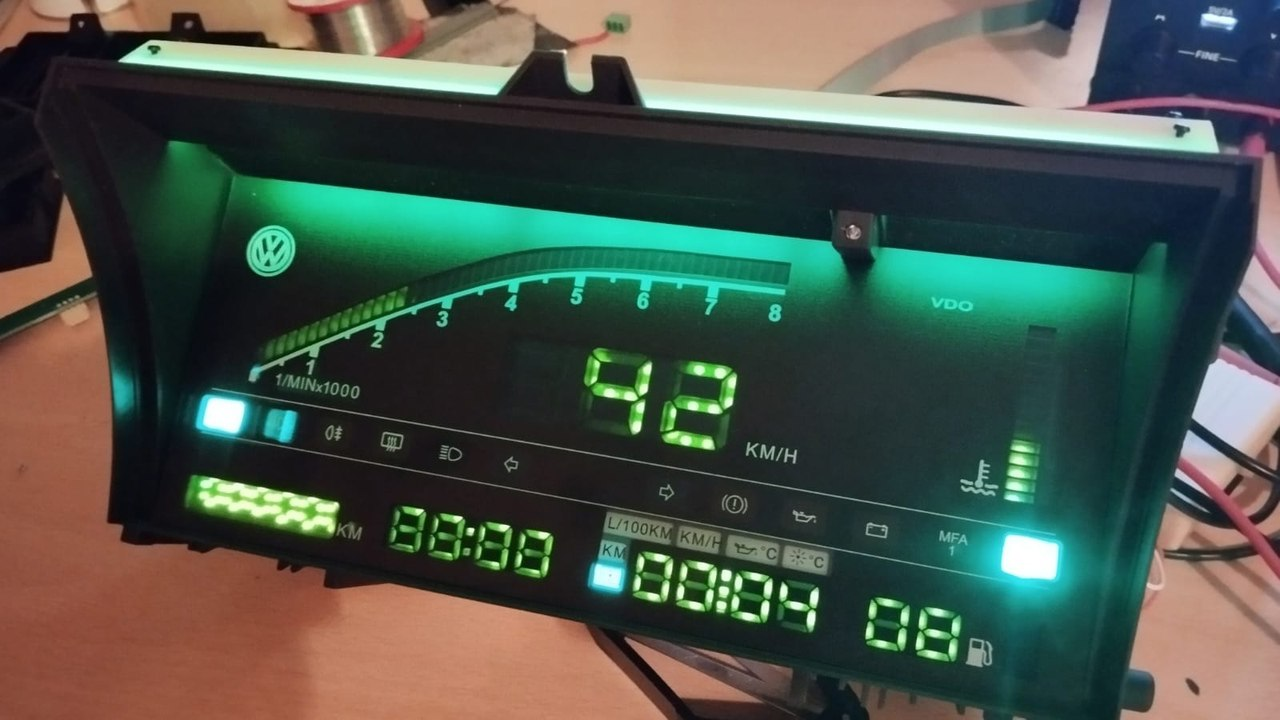
\includegraphics[width=\linewidth]{digifiz_manual/image047.png}
        \caption{Round-edge fascia used on later kits.}
    \end{subfigure}
    \caption{Aspecto del cuadro \ReplicaGenOne{}.}
    \label{fig:replica-classic}
\end{figure}

\section{Manipulación y cuidado de la pantalla}
\begin{itemize}
    \item La parte frontal de plexiglás con impresión UV se marca con facilidad. Evite el contacto con objetos punzantes o abrasivos.
    \item Los daños superficiales son cosméticos y no están cubiertos por la garantía. Solicite piezas de repuesto a PHOL-LABS Kft si el patrón de la pantalla se deforma.
\end{itemize}

\section{Batería del reloj en tiempo real}
El cuadro incorpora un reloj en tiempo real DS3231 con una pila CR2032. La batería suele durar alrededor de cuatro años. Cuando se agota, el reloj se reinicia en cada encendido. Retire la tapa frontal y/o trasera, mantenga conectados los mazos de cables y sustituya la pila tipo botón. Deseche la batería usada según la normativa local.

\section{Mantenimiento de firmware con USBasp}
Cada kit se entrega con un cable de programador USBasp ya conectado dentro de la carcasa (\autoref{fig:usbasp-cable}). Instale un controlador USBasp adecuado antes de grabar. Por ejemplo, descárguelo en la siguiente dirección:
\displayurl{https://myrobot.ru/downloads/driver-usbasp-v-2.0-usb-isp-windows-7-8-10-xp.php}
El programador alimenta el cuadro cuando se conecta a un ordenador, lo que permite realizar pruebas en banco.

\begin{figure}[htbp]
    \centering
    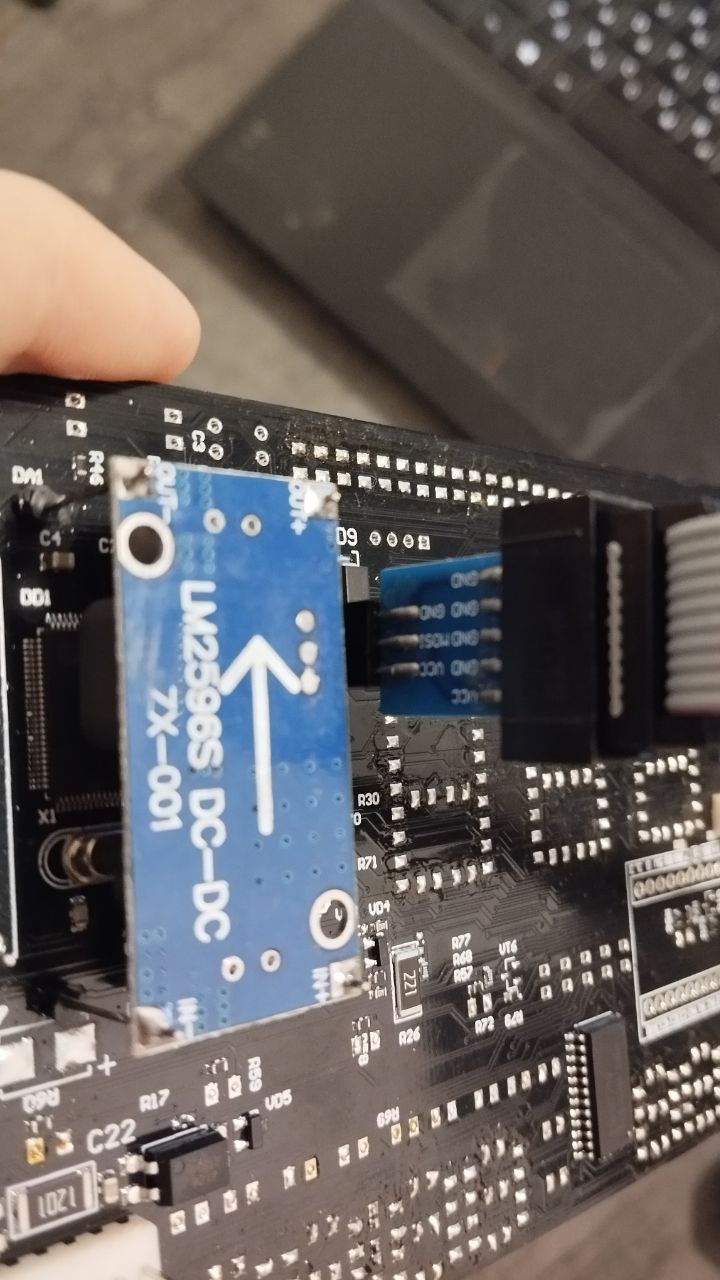
\includegraphics[width=0.32\textwidth]{digifiz_manual/image048.png}
    \caption{Orientación del mazo USBasp dentro del \ReplicaGenOne{}.}
    \label{fig:usbasp-cable}
\end{figure}

Grabe el firmware con \texttt{avrdude} mediante el comando siguiente (sustituya el nombre del archivo si es necesario):

\begin{verbatim}
avrdude -c usbasp -p m2560 -e \
    -U lfuse:w:0xff:m -U hfuse:w:0x99:m -U efuse:w:0xff:m \
    -U flash:w:Digifiz.ino.mega.hex
\end{verbatim}

Después de una carga correcta pulse el botón táctil frontal cuatro o cinco veces para inicializar los bloques de memoria. Si los bloques siguen vacíos, repita el proceso de grabación o envíe el comando Bluetooth \verb|252 0| para ejecutar un restablecimiento de fábrica. Las imágenes de firmware listas para usar se publican en:
\displayurl{https://github.com/Sgw32/DigifizReplica}

\section{Configuración por Bluetooth}
La mayoría de los parámetros se ajustan mediante Bluetooth usando un teléfono Android y la aplicación Serial Bluetooth Terminal. Descárguela del enlace siguiente antes de emparejar con el cuadro:
\displayurl{https://play.google.com/store/apps/details?id=de.kai_morich.serial_bluetooth_terminal&hl=en&gl=US}
Los dispositivos iOS no pueden conectarse al módulo Bluetooth 2.0 clásico.

\begin{itemize}
    \item Ensure you pair with the dashboard's Bluetooth Classic interface rather than BLE-only devices.
    \item In Serial Bluetooth Terminal set the end-of-line character to LF. Disable CR+LF before sending commands.
\end{itemize}

\begin{figure}[htbp]
    \centering
    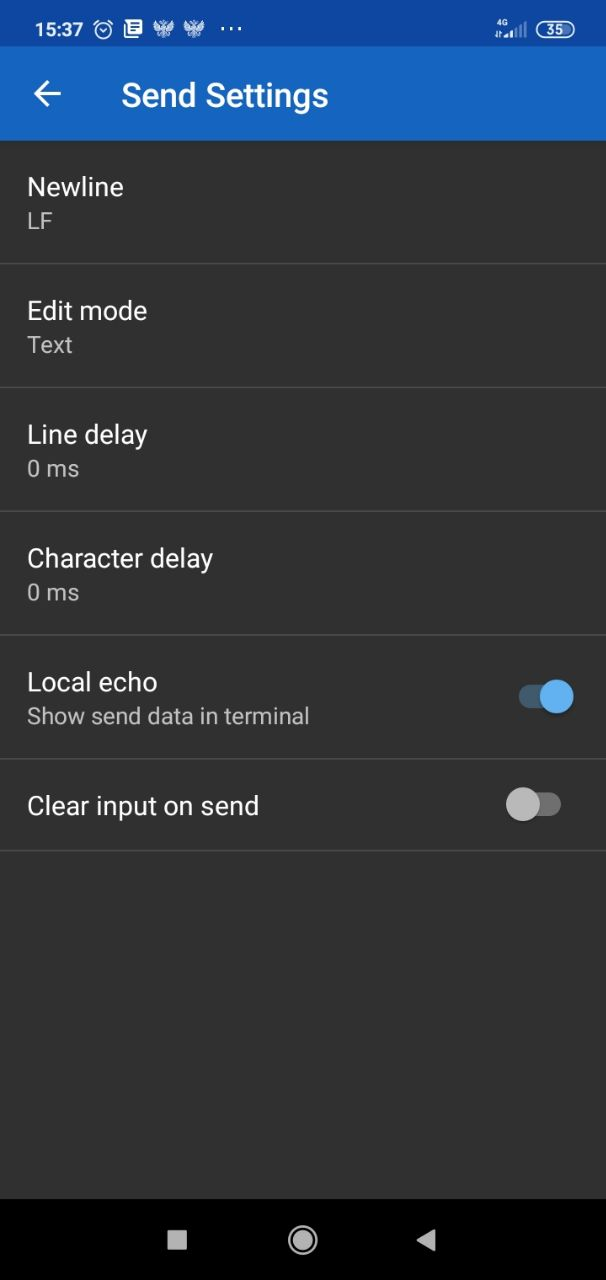
\includegraphics[width=0.32\textwidth]{digifiz_manual/image049.png}
    \caption{Configuración recomendada de Serial Bluetooth Terminal.}
    \label{fig:sbt-settings}
\end{figure}

Introduzca los comandos como pares separados por espacios \verb|<número> <valor>|. Por ejemplo, para guardar un odómetro de 123\,456~km envíe \verb|11 123456|. Sume 128 al número de comando para leer su valor actual (\verb|129 0| devuelve el coeficiente de velocidad). El comando de diagnóstico \verb|adc 0| muestra lecturas sin procesar de los sensores que ayudan a los desarrolladores a analizar fallos.

\section{Parámetros de configuración}
Los comandos Bluetooth principales se enumeran en \autoref{tbl:replica-classic-commands}. Los ajustes predeterminados para los cuadros de las generaciones~1/1.5 y~2 se resumen en \autoref{tbl:replica-defaults}. Utilice los comandos~31--33 solo en unidades \ReplicaNextShort{}; no tienen efecto en el \ReplicaGenOneShort{} clásico.

{\scriptsize
\begin{longtblr}[
    caption = {Comandos de configuración del \ReplicaGenOne{} clásico.},
    label = {tbl:replica-classic-commands},
]{
    colspec = {Q[c,0.14\linewidth] >{\ttfamily}Q[l,0.38\linewidth] Q[l]},
    rowsep = 2pt,
}
    \toprule
    \textbf{ID} & \textbf{Nombre} & \textbf{Descripción} \\
    \midrule
    22 (o 0) & PARAMETER\_RPMCOEFFICIENT & Factor de calibración de RPM del motor. \\
    1 & PARAMETER\_SPEEDCOEFFICIENT & Factor de calibración de velocidad. \\
    2 & PARAMETER\_COOLANTTHERMISTORB & Coeficiente beta del termistor de refrigerante. \\
    3 & PARAMETER\_OILTHERMISTORB & Coeficiente beta del termistor de aceite. \\
    4 & PARAMETER\_AIRTHERMISTORB & Coeficiente beta del termistor ambiente. \\
    5 & PARAMETER\_TANKMINRESISTANCE & Resistencia mínima del aforador (\si{\ohm}). \\
    6 & PARAMETER\_TANKMAXRESISTANCE & Resistencia máxima del aforador (\si{\ohm}). \\
    7 & PARAMETER\_TAU\_COOLANT & Constante del filtro de temperatura de refrigerante. \\
    8 & PARAMETER\_TAU\_OIL & Constante del filtro de temperatura de aceite. \\
    9 & PARAMETER\_TAU\_AIR & Constante del filtro de temperatura ambiente. \\
    10 & PARAMETER\_TAU\_TANK & Constante del filtro de nivel de combustible. \\
    11 & PARAMETER\_MILEAGE & Valor total del odómetro. \\
    12 & PARAMETER\_DAILY\_MILEAGE & Odómetro parcial. \\
    13 & PARAMETER\_AUTO\_BRIGHTNESS & Activar ajuste automático de brillo. \\
    14 & PARAMETER\_BRIGHTNESS\_LEVEL & Nivel de brillo manual (0--15). \\
    15 & PARAMETER\_TANK\_CAPACITY & Capacidad del depósito (litros). \\
    16 & PARAMETER\_MFA\_STATE & Página MFA activa. \\
    17 & PARAMETER\_BUZZER\_OFF & Desactivar el zumbador (1 desactiva, 0 habilita). \\
    18 & PARAMETER\_MAX\_RPM & Escala del cuentarrevoluciones (8000 por defecto). \\
    19 & PARAMETER\_NORMAL\_RESISTANCE\_COOLANT & Resistencia del sensor de refrigerante a \SI{25}{\celsius}. \\
    20 & PARAMETER\_NORMAL\_RESISTANCE\_OIL & Resistencia del sensor de aceite a \SI{25}{\celsius}. \\
    21 & PARAMETER\_NORMAL\_RESISTANCE\_AMB & Resistencia del sensor ambiente a \SI{25}{\celsius}. \\
    23 & PARAMETER\_DOT\_OFF & Comportamiento de los dos puntos del reloj (0 parpadeo, 1 fijo). \\
    24 & PARAMETER\_BACKLIGHT\_ON & Encender la retroiluminación con las luces de cruce. \\
    25 & PARAMETER\_M\_D\_FILTER & Constante del filtro mediano (heredado). \\
    26 & PARAMETER\_COOLANT\_MAX\_R & Umbral de temperatura de refrigerante para escala completa. \\
    27 & PARAMETER\_COOLANT\_MIN\_R & Umbral de temperatura de refrigerante para ``1~bar''. \\
    31--33 & PARAMETER\_MAINCOLOR\_[RGB] & Componentes de color de la interfaz (solo \ReplicaNextShort{}). \\
    37 & PARAMETER\_RPM\_FILTER & Intensidad del filtrado de RPM. \\
    128 & PARAMETER\_READ\_ADDITION & Sumar para leer cualquier parámetro. \\
    255 & PARAMETER\_SET\_HOUR & Ajustar horas del reloj (formato 24 h). \\
    254 & PARAMETER\_SET\_MINUTE & Ajustar minutos del reloj. \\
    253 & PARAMETER\_RESET\_DAILY\_MILEAGE & Restablecer el odómetro parcial. \\
    252 & PARAMETER\_RESET\_DIGITAL & Restablecimiento de fábrica e inicialización de memoria. \\
    \bottomrule
\end{longtblr}}

Los botones rápidos de Serial Bluetooth Terminal son prácticos para acciones habituales como activar o desactivar el brillo automático (\verb|13 0| y \verb|13 1|) o escribir valores de color. Mantenga valores de brillo por encima del \SI{60}{\percent} solo durante pruebas breves para preservar la vida útil de los LED.
